\documentclass{beamer}

\usepackage{amsmath, amssymb}
\usepackage{tikz-cd}
\usepackage{xcolor}
\usepackage{graphicx}

\title{MAT434: Theory of Mathematical Statistics}
\author{\textbf{Miraj Samarakkody}}
\institute{Tougaloo College}
\date{02/12/2025}

\begin{document}

\begin{frame}
    \titlepage
\end{frame}

\begin{frame}{The Binomial Distribution}
    Suppose the \(n\) independent experiments are performed, each resulting in a success with probability \(p\). Let \(X\) be the number of successes in the \(n\) experiments.\\
    \vspace{0.1in}
    \pause
    The probaility that \(p(k)\) can be found in the following way:\\
    \vspace{0.1in}\pause
    Any particular sequence of \(k\) successes and \(n-k\) failures has probability \(p^k(1-p)^{n-k}\) from the multiplication principle. \\
    \pause
    \vspace{0.1in}
    The number of such sequences is \(\binom{n}{k}\).\\\pause
    \vspace{0.1in}
    Thus \[
    P(X=k)=p(k)=\binom{n}{k}p^k(1-p)^{n-k}
    \]

\end{frame}

\begin{frame}{Example}
    Let \(n=10\) and \(p=0.1\). \pause
    \begin{figure}
        \centering
        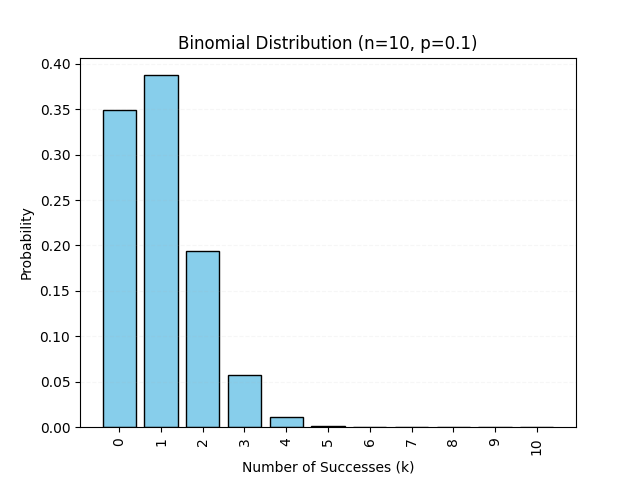
\includegraphics[width=0.5\textwidth]{Figures/Figure_1.png}
        \caption{The Binomial Distribution for \(n=10\) and \(p=0.1\)}
        \label{fig:binomial1}
    \end{figure}
\end{frame}

\begin{frame}{Example}
    Let \(n=10\) and \(p=0.5\). \pause
    \begin{figure}
        \centering
        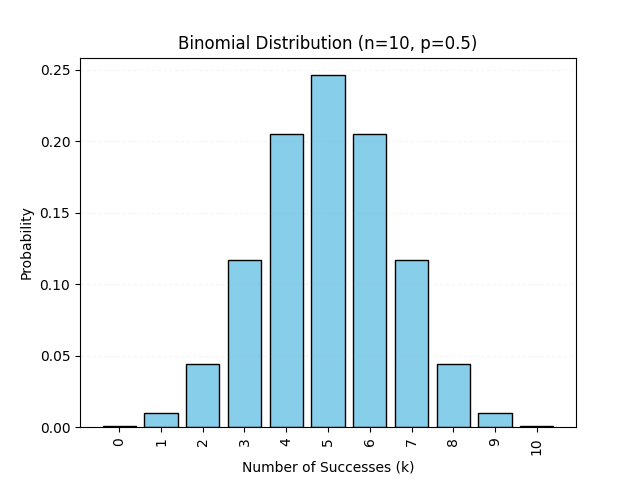
\includegraphics[width=0.5\textwidth]{Figures/Figure_2.png}
        \caption{The Binomial Distribution for \(n=10\) and \(p=0.5\)}
        \label{fig:binomial2}
    \end{figure}
\end{frame}

\begin{frame}{Example}
    Let \(n=10\) and \(p=0.8\). \pause
    \begin{figure}
        \centering
        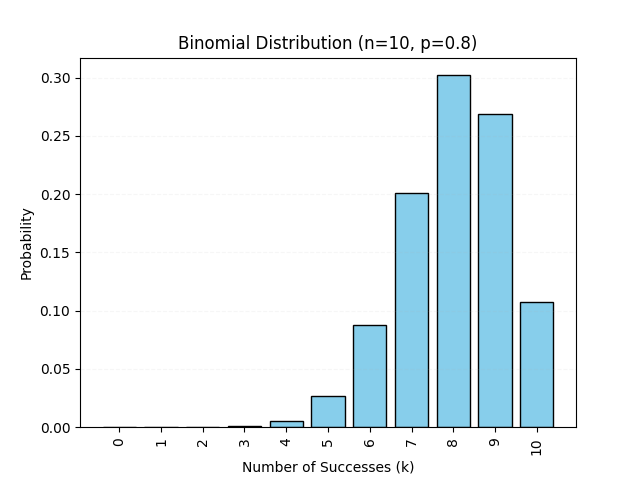
\includegraphics[width=0.5\textwidth]{Figures/Figure_3.png}
        \caption{The Binomial Distribution for \(n=10\) and \(p=0.8\)}
        \label{fig:binomial3}
    \end{figure}
\end{frame}

\begin{frame}{The Geometric and Negative Binomial Distribution}
    \begin{block}{The Geometric Distribution}
        The geometric distribution if also constructed from independent Bernoulli trials, but from an infinite sequence. \pause
        \vspace{0.1in}
        On each trail, a success occurs with probability \(p\), and \(X\) is the total number of trials up to and including the first success. \pause
        \vspace{0.1in}
        From the indepedance of the the trails, this occurs with probability \[
                p(k)= P(X=k)=(1-p)^{k-1}p, ~~k=1,2,3, \dots
        \]
    \end{block}\pause
    Note that these probabilities sum to 1. \[
    \sum_{k=1}^{\infty} (1-p)^{k-1}p = p \sum_{j=0}^{\infty}(p-1)^j=1
    \]
\end{frame}

\begin{frame}{Example}
    The probability of wining a certain state lottery is said to be about \(1/9\).\pause\\
    If it is exactly \(1/9\), the distribution of the number of tickets a person must purchase up to and including the first wining ticket is geometric random variable with \(p=1/9\).\pause
    \begin{figure}
        \centering
        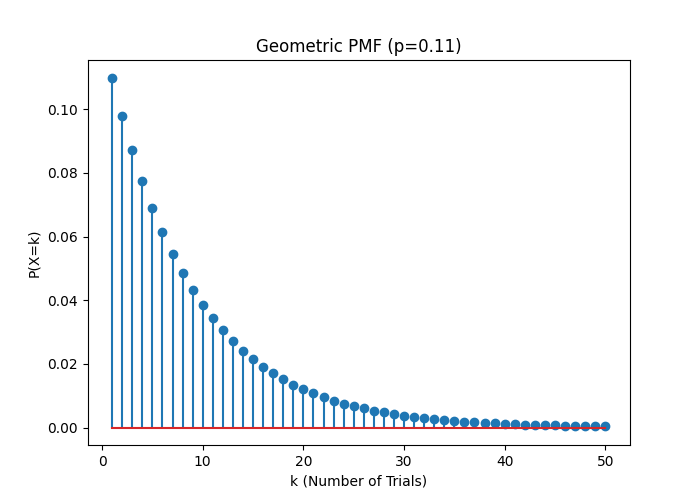
\includegraphics[width=0.5\textwidth]{Figures/Figure_4.png}
        \caption{The probability mass function of a geometric random variable with \(p=1/9\)}
        \label{fig:geometric1}
    \end{figure}
\end{frame}

\begin{frame}
    \frametitle{Negative Binomial Distribution} 
\begin{block}{Negative Binomial Distribution}
    
\end{block}
    

\end{frame}


\end{document}